%!TEX root = ../../super_main.tex

\chapter{Evaluation}
\label{cha:quality_assurance}

This chapter describes some of the different measures we have used in order ensure the quality of uMiner. This chapter will also cover some reflections in regards to the way we have used, and gained from, different tools and techniques, such as continuous integration, unit tests, manual test, and general product evaluation through fellow software engineering students and  people outside this category. 
\\\\
When executing any dynamic test, i.e. tests that runs code on some device, we tried to run it on as many devices as possible. This was done in order to test our system on different hardware configurations and over different Android versions.

%!TEX root = ../../super_main.tex

\section{Continuous Integration}
\label{sec:continuous_integration}
As mentioned in \secref{sec:extreme_programming}, we wanted a Continuous Integration (CI) server in order to ensure that our code base always was at a stable state. We installed Jenkins on the same server that makes up the server part of our client-server architecture because it was easily available. Jenkins is an open source automation server, which supports various different plugins that helps with builds, viewing test results, etc. We configured this Jenkins server to be notified whenever our Git version control code repositories (hosted on GitHub) for both Android and PHP code were changed. When this notification happened, Jenkins would build the corresponding project and automatically run its unit tests. Whenever the build projects would go from a previously successful build to a now failing build or vice versa, the Jenkins system would send out mails to our group, so we were aware that something went wrong or that it was now fixed again. If a build failed, the mail would contain information regarding which tests failed, and their stack trace. This made it possible for us to give immediate attention to issues that we did not catch before pushing our content to the version control. \figref{fig:jenkins_front_page} shows the front page of the Jenkins website. In the left side, the build queue can be seen, which shows if any builds are currently running. In the center, the various projects that are currently configured for the Jenkins setup can be seen. The blue circle changes to red if the most recent build was a failure, and besides that, it can be seen how long time has passed since the most recent pass, most recent failure, and how long the last build took to finish. By clicking on one of the projects, statistics can be seen for checkstyes warnings, code coverage, and test results. 

\begin{figure}[!htbp]
    \centering
    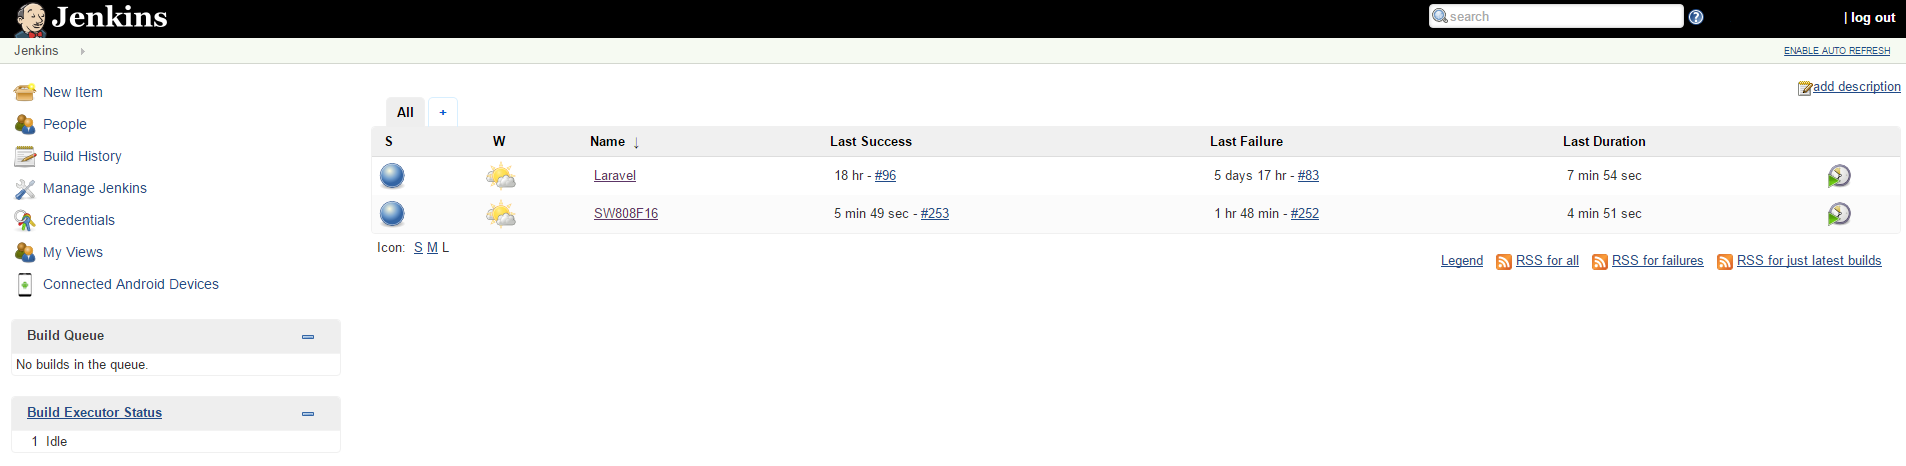
\includegraphics[width=\textwidth]{graphic/quality_assurance/jenkins_frontpage}
    \caption{Jenkins CI front page.}
    \label{fig:jenkins_front_page}
\end{figure}
\FloatBarrier

We used this extensively during the development, because when several people merge their work into the master branch of the version control several times per day, something is bound to go wrong eventually. This ensured that we always knew if something was wrong with either of our projects, so we knew when we needed to allocate people for fixing it. 


%!TEX root = ../../super_main.tex

\section{Code Metrics}
\label{sec:automated_unit_test}

Our development method states that all code we develop should be made in a test-first fashion (see \secref{sec:extreme_programming}). We therefore attempted to always make test cases for all the features we implemented. Our code coverage graphs can be seen in \figref{fig:android_project_code_coverage} and \figref{fig:php_project_code_coverage}, for our Android and PHP projects respectively. The two figures look different because we use different plugins on the CI server (due to the projects being written in different programming languages). We could have used a more strict coverage metric than line coverage, but due to prioritization of feature development we have chosen not to. Other interesting and useful coverage metrics includes branch coverage. In the Android project our line coverage percentage is $\sim 43\%$, which is relatively low. %But as explained previously, this is due to the complexity of the integration tests which were manual instead. 

% In \figref{fig:android_project_code_coverage} the line coverage is represented with green while missed lines are represented with red. In \figref{fig:php_project_code_coverage} the red line is method coverage, blue is line coverage and green is total.

\begin{figure}[!htbp]
    \centering
    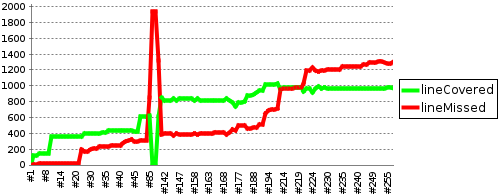
\includegraphics[width=0.7\textwidth]{graphic/quality_assurance/jenkins_android_code_coverage}
    \caption{Android project code coverage}
    \label{fig:android_project_code_coverage}
\end{figure}
\FloatBarrier

In the PHP project, we have a $\sim 74\%$ line coverage, which is rather good. Most of the untested code is library- or auto generated code, and we have not tested this because we assume these parts work as they are supposed to. This is a risk assessment we have made, and deemed insignificant, in contrast to the speed we gain from using the libraries without testing them. % If we only considered coverage on the code we made ourselves, it would probably exceed 90\%. 

\begin{figure}[!htbp]
    \centering
    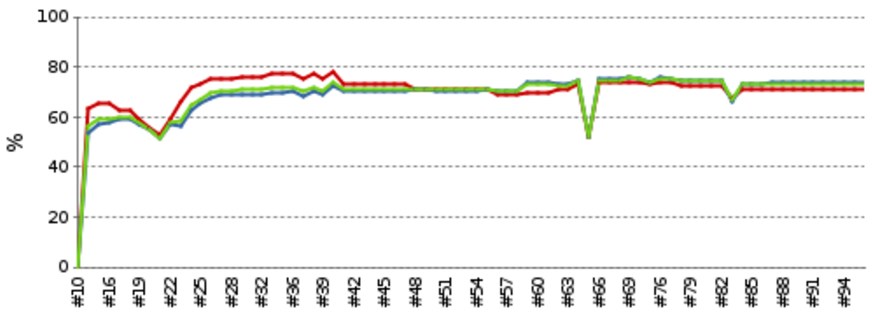
\includegraphics[width=0.7\textwidth]{graphic/quality_assurance/jenkins_php_code_coverage}
    \caption{PHP project code coverage}
    \label{fig:php_project_code_coverage}
\end{figure}
\FloatBarrier

\subsection{Manual Test}
In some cases it was infeasible to create automatic dynamic white box tests in decent time, and we therefore, in these cases, switched to a dynamic black box approach instead. Here we made test specifications, executed some part of the code manually and observed the result relative to the specifications. We mainly did this for the more complex parts of the code, such as the \mono{BackgroundSensorService} class, which schedules all the \mono{SensorProvider}s asynchronously and sends the results to the server. Here we test if the sensor provider outputs the data correctly to the server. We also used this approach for other testing methods, such as regression and integration testing of UI features. For instance, we would, when a new UI-related feature was implemented, manually test if previous UI features still worked. We did not spend time on specifying written test-cases on the most basic integration tests, such as ``is it possible to subscribe to a campaign?'', since these would probably be found during ad-hoc testing done while developing new features.
\\\\
These manual tests resulted in a generally lower line coverage, especially on the Android project, since the CI plugin we used was unable to compare our manual tests to the code base. This does not necessarily mean that the code is less tested, but it is harder to tell when tests are covering the code base well. 

\subsection{Static Code Analysis}
Besides using coverage metrics, we have used some metrics produced by static code analysis to improve the quality of our code base. We have used a linter, which will produce warnings on code that is known to be error prone, which helps us avoid common mistakes on the Android platform and Java in general. Furthermore, we have used check-style, which helps us find structural inconsistencies in our code base. Effectively, this type of metric will assist us in keeping our code base uniform and look consistent, which will make it easier for all developers to read the code, since all parts of the code base is structured in the same way.


%!TEX root = ../../super_main.tex

\section{Testing Platform}
\label{sub:testing_platform}

At first in our development process, we utilized JUnit tests for testing the native Android code. However, alot of different features in the Android framework are specific to Android and are not testable using JUnit, because it is a tool originally designed for standard Java development. To solve this problem we aditionally chose to utilize the Robolectric framework\footnote{http://robolectric.org/} , which allows for mocking of Android \emph{Activity} objects and general Android behavior from the native environment when using JUnit. This allows very coupled Android components to be tested seperately and without the use of an emulator or an actual device. 
\\\\
That worked until we started using sensors during the development, because neither the JUnit framework nor the Robolectric framework facilitate mocked sensor events. Sensor events were an important part of the solution we had in mind, and we therefore decided to start using instrumented tests, which is tests that is run on an Android device. This could easily be facilitated during the development by using our own Android cellphones, but for the purpose of Continuous Integration and Jenkins builds, the server also needed access to a running device. It would be inconvenient to use our own phones, because the server had to be located in the basement of the institute in order to have access from outside the university's network. 
\\\\
The mobile telephones we could borrow from the university were old devices running Android version 4.3 or lower, which correspond to Android API level 18 \parencite{uses_sdk}. Since only roughly a quarter of Android devices run this version or lower \parencite{android_dashboard} we deemed that it was too unused. Furthermore, newer versions of Android were improved and provided many new features related to wearables, which appealed to us. Meanwhile most of the phones in the group was API level 21 or higher, we therefore chose API level 21 as the minimum supported version. 
\newpage
This meant that in order to use the devices we could borrow, we had to root them and flash a new OS onto them. The devices we could borrow were the Galaxy S3 Mini VE (i8200) and the Galaxy S3 Mini (i8190). We spent a couple of days on researching and attempting to install a newer Android OS on the two devices, but the i8200 did not have any ROMs available from trustworthy sites, and the i8190 would enter a boot-loop when we flashed it. Both phones were therefore reset to factory settings and returned. After this we got our hands on a Galaxy Nexus, for which the Android community has made a lot of high quality ROMs and guides for flashing. We managed to flash the Nexus to 5.0 (API 21), which allowed us to connect it to the CI server and run instrumented tests. We therefore decided to migrate all of our old Robolectric tests to instrumented tests, such that we only had a single type of tests. 


%!TEX root = ../../super_main.tex

\section{Monkey Test}
\label{sec:monkey_test}
We executed UI/Application Exerciser Monkey tests on the android code. The exerciser monkey generates pseudo-random streams of user events, which can be used to test the robustness of the application. The monkey is able to stress-test the application because of frequent button clicks, etc., such that it most likely crashes if there are memory leaks or other bad implementations. It furthermore provides the possibility of simulating erratic user behavior, that might perform some trace of actions that human users would not typically follow, which might crash the application. Whenever the monkey crashes the application, the entire trace is available, but we mainly used it for the crash reports and exceptions that are available through the Android Debug Bridge. 
\\\\
We started by running one trace on 50000 inputs on a Galaxy Nexus phone, where the application crashed after 46000 actions, which allowed us to take a look at the exception and resolve it. Afterwards the monkey ran for 2 hours straight without crashing, and we therefore think the application is rather robust.
\\\\
Following this we also ran the monkey for a while on a Nexus 5 device which had Android 6.x, in contrast to the 5.x on the Galaxy Nexus. Here it also seemed to run without any difficulties, which gives some indication that our application is resilient in terms of different configurations and also compatible with different versions of Android without issues.
\\\\
We have also been using the monkey to discover cases where, if you executed a certain set of actions fast enough, it would would result in incorrect application behavior. This includes things such as subscribing to a campaign, immediately exiting the menu and then entering the same menu again, where the communication between application and server had not finished registering the participant yet. This allows us to find certain use patterns that we need to consider, or at least need to keep in mind, even if we do not have solutions for them at the time.
\\\\
It is also possible to configure CI servers to run automated monkey tests if so desired, but we did not think this was a good idea for our project. This was partially because it takes quite a bit of time to execute the monkey test, but also because it has access to the settings of the phone, which might mess up the unit tests. So given the amount of precautions, resets, etc., that might be necessary, we deemed it to take too much time to set up. 


%!TEX root = ../../super_main.tex

\section{Pair Group Review}
\label{sec:pair_group_review}

Two times during the project period we arranged meetings with another group of software students at Aalborg University, where we presented the current states of our projects and provided critique for each other. One meeting was arranged halfway through the semester and another was arranged three weeks before project delivery. 

\subsection{First Meeting: Project Idea}
\label{sub:first_meeting_project_idea}
The goal of the first meeting was to evaluate the general project idea of the opponent group and also suggest improvements for the developed system. At this meeting the two groups were unfamiliar with the product of the other group, so an agenda was created that should increase the understanding for the opponent:

\begin{itemize}
    \setlength\itemsep{-0.2em}
    \item Introduction
    \item Demonstration
    \item Evaluation
\end{itemize}

We took turns in presenting, so the first group started by introducing their problem area, how they were going to solve the problem and which customers might be interesting in using the developed product. After the presentation of the problem area, the group presented the current state of the product, which was followed by two different evaluations from the opponent group. One evaluation was regarding the idea and the marketability of the solution, while the other was regarding how the product could be improved. 
\\\\
The result of this meeting were mainly on the idea level, and not so much about the product specifically. Our opponent group had concerns regarding how we were going to persuade participants to use the system, such that we could actually gather the data that we claimed would be available for our customers. We decided that this was not a big concern, since the customers would be interested in branding their campaigns in order to find and persuade participants to contribute. In any case, we think that we provide a platform for customers to use, so that they only have to provide some incentive for participants to join, is an improvement in itself. We furthermore hope that the participants who join for the rewards of the branded campaigns would be interested in selecting campaigns that only offered small or no rewards. We think it is realistic to assume, that if customers do not offer any rewards whatsoever on their own without our system, they would probably not get any participants anyway. 

\subsection{Second Meeting: Product Evaluation}
\label{sub:second_meeting_product_evaluation}

At the second meeting, both the groups' products were in an nearly finished state, and were presented for the other group. The goal of this meeting was to determine if there were any obscure parts of the system, bugs, possible usability improvements or extensions to the system. Our opponent group could not find any bugs in the system, but they suggested some potential usability improvement and an extension that would be nice to have in the system. The suggestions are represented in \tabref{tab:suggestions_from_opponent_group}. 

\begin{table}[!htbp]
    \centering
    \begin{tabular}{|l|p{0.8\textwidth}|}
    \hline
    \textbf{Category} & \textbf{Description} \\ \hline
    Extension & Run questionnaires at specific times of the day, instead of relative to time of joining campaign.  \\ \hline
    Usability & Put the definition of our time intervals on the website, or show it with an image. \\ \hline
    Usability & Move the active campaign to the top of the campaigns list instead of where it was located before. \\ \hline
    Usability & Have focus on the size differences on the website. Many items are rather small, so it is hard to determine what is important. The most important things should be large. \\ \hline
    \end{tabular}
    \caption{Suggestions from opponent group.}
    \label{tab:suggestions_from_opponent_group}
\end{table}

These were all valid suggestions, but due to the meeting being held a bit too close to the project deadline, we had to prioritize documenting our work over furhter development. Effectively, this resulted in only the second entry being implemented: \emph{Put the definition of our time intervals on the website, or show it with an image}. There is now an image on the website which represents how to understand the different intervals you can specify on the ``create campaign''-site. The other three entries are things that would be nice improvements to the system, and definitely something that should be worked on, if the system was to be extended at some point. 


%!TEX root = ../../super_main.tex
\section{Participant Experience Evaluation}
\label{sec:participant_experience_evaluation}

We want uMiner to be as general as possible in terms of who participants might be. Meaning that we want to target as many different personas as possible in terms of user experience of the Android application. We have for this reason tried to create some sort of user experience evaluations in regards to the part of the system the participants are going to use. The idea of this evaluation is to determine if there are some obvious flaws in the design of how our Android application in regards to disturbing the participants. We want to investigate if we developed a solid start for part of the client application that notifies and asks the participants questions. This evaluation was performed with five people having a compatible smartphone, firstly this is not a great deal of test subjects and does not provide any statistical evidence for the evaluation of the system, but we hope to get some constructive evaluation of the application never the less. Furthermore one should not that the persona of these five test subjects are rather similar. All five are male in their start 20s, with similar interests, all being tech savvy some extend.

\subsection{Setup}
\label{sub:setup}

We have created a test campaign called ``Alcohol and you'' which should emulate the type of campaign a final customer might specify. The campaign specification can be seen in \tabref{tab:test_campaign_spec}. This specification means that we take 600 measurements every hour and we desire answers for a questionnaire every other hour.

\begin{table}[!htbp]
    \centering
	\begin{tabular}{|m{0.3\textwidth}|m{0.7\textwidth}|} \hline
	Total duration        & 2 hour            \\ \hline
	Sample frequency      & 1 minute          \\ \hline
	Sample duration       & 2 seconds         \\ \hline
	Measurement frequency & 200 miliseconds   \\ \hline
	Sensors               & \begin{itemize}[noitemsep]
								\item Accelerometer 
								\item Ambient Light
								\item Barometer
								\item Compass
								\item Gyroscope
								\item Location
								\item Proximity
								\item Galvanic Skin Response (Microsoft Band 2)
								\item Heartbeat (Microsoft Band 2)
							\end{itemize}                \\ \hline
	Questions             & \begin{itemize}[noitemsep]
								\item Have you within the last two hours had an alcoholic beverage?
								\item Have you within the last two hours had a carbonated alcoholic beverage?
								\item Have you within the last two hours had a strong alcoholic beverage with (more than 10\% alcohol)?
								\item Do you feel influenced by alcohol?
							\end{itemize}                \\ \hline
	\end{tabular}
	\caption{Alcohol and you specification}
	\label{tab:test_campaign_spec}
\end{table}
\FloatBarrier

The application was distributed and installed on devices of test subjects, and they were guided to how they could start contributing to our test campaign. This means that this test does not in any way evaluate the main activity of the system, it only evaluates the experience of being notified by the application and prompted with questions. After the setup of the application we told the test subjects to proceed with their daily life and treat the uMiner application as any other application the might have installed from the Google Play Store. 

\subsection{Results}
\label{sub:results}
After 24 hours of the application being installed on the test participants devices we asked them a series of questions to understand the disturbance of the notifications and questionnaire throughout one day of experience. The results of this survey can be seen in \tabref{fig:survey_results}. These results show that our participants in general are not being disturbed to a severe degree. Most of the participants did answer they was not distrubed at all as seen in \figref{fig:general_disturbance}, where the one person feeling disturbed only deemed it to be a degree 2 out of 5 of disturbance as seen in \figref{fig:disturbance_level}. Same goes for the amount of notifications being dismissed, as seen in \figref{fig:ingore_notifications}, only 1 in 5 ignored the notifications and they only did so for half of them or less. Lastly none of the test participants had the desire to uninstall the application after contributing for a day as seen in \figref{fig:want_to_uninstall}.


\begin{figure}[!htbp]
    \begin{subfigure}[!t]{.45\textwidth}
      \centering
        %!TEX root = ../../../super_main.tex
\pgfplotstableread[row sep=\\,col sep=&]{
    interval & disturbance\\
    1   & 0  \\
    2   & 0  \\
    3   & 1 \\
    4   & 2 \\
    5   & 2 \\
    }\mydata
\begin{tikzpicture}
    \begin{axis}[
            width  = \textwidth,
            height = 5.5cm,
            ymax=5,
            ytick={0,1,2,3,4,5},
            nodes near coords,
            ybar,
            symbolic x coords={1,2,3,4,5},
            xtick=data,
        ]
        \addplot table[x=interval,y=disturbance]{\mydata};
    \end{axis}
\end{tikzpicture}
        \caption{On a scale from 1 to 5, where 1 is novice and 5 is expert how would you rate your abilities to utilize a smartphone.}
      \label{fig:smartphone_ability}
    \end{subfigure}
    ~
    \begin{subfigure}[!htbp]{.45\textwidth}
      \centering
        %!TEX root = ../../../super_main.tex
\begin{tikzpicture}
\pie[text=legend, radius=2, sum=auto, after number=]
{
  1/Yes, 
  4/No
}
\end{tikzpicture}
      \caption{Did you feel that the application was disturbing?}
      \label{fig:general_disturbance}
    \end{subfigure}
    \vspace{1em}
    \begin{subfigure}[!htbp]{.45\textwidth}
      \centering
        %!TEX root = ../../../super_main.tex
\pgfplotstableread[row sep=\\,col sep=&]{
    interval & disturbance\\
    1   & 0  \\
    2   & 20  \\
    3   & 0 \\
    4   & 0 \\
    5   & 0 \\
    }\mydata
\begin{tikzpicture}
    \begin{axis}[
            width  = \textwidth,
            height = 5.5cm,
            ybar,
            nodes near coords,
            ymax=100,
            symbolic x coords={1,2,3,4,5},
            xtick=data,
        ]
        \addplot table[x=interval,y=disturbance]{\mydata};
    \end{axis}
\end{tikzpicture}
      \caption{On a level from 1 to 5, to what degree did you feel disturbed?}
      \label{fig:disturbance_level}
    \end{subfigure}
    ~
    \begin{subfigure}[!htbp]{.45\textwidth}
      \centering
        %!TEX root = ../../../super_main.tex
\begin{tikzpicture}
\pie[text=legend, radius=2,sum=auto, number =]
{
  1/Less than half, 
  4/None
}
\end{tikzpicture}
      \caption{How many of the notifications uMiner sent did you ignore of dismiss?}
      \label{fig:ingore_notifications}
    \end{subfigure}
    \vspace{1em}
    \begin{subfigure}[!htbp]{\textwidth}
      \centering
        %!TEX root = ../../../super_main.tex
\begin{tikzpicture}
\pie[text=legend, radius=2, sum=auto, after number=]
{
  5/No
}
\end{tikzpicture}
      \caption{Did you at any point want to uninstall the application?}
      \label{fig:want_to_uninstall}
    \end{subfigure}
    \caption{Survey results.}
    \label{fig:survey_results}
    \end{figure}
\FloatBarrier

In this small set of test participants the general user experience regarding the notifications and questionnaires showed to be rather successful. Besides these metrics in \figref{fig:survey_results}, we got some feedback for the application concerning the fact that we ask the same question multiple times throughout a day. One of the participants sent the following feedback:

\begin{quote}
    \translated{If i was not drunk at 6.20 in the morning, i am probably not drunk at 8 or 10 either.}
\end{quote}

We can see the concern of this participant, and could imagine that the questionnaires would be rather tedious to answer because the user is prompted for the exact same thing over and over. One could imagine that platform would have to provide a better way of prompting for questions, for instance only ask questions once a day. With the ``Alcohold and you'' campaign, one could imagine that the user was asked daily with something like, ``Have you consumed alcohol today?'', and then give the user to enter some timespan in where he was influence by alcohol. However with this approach the accuracy of the snapshots rely on the memory of the participants and this might pollute the snapshots with less accurate data. The important thing to consider is that if the platform should be further developed it is important that it provides great tools for the customer to specify on how he wants to ask the participants questions. 
\\\\
In the end the customer want to get as accurate data as possible while still disturbing the participants as little as possible, it will be a challenge to maintain both of these qualities or find some good trade-off between them.

%!TEX root = ../../super_main.tex

\section{Data Usefulness}
\label{sec:data_usefulness}

We need to investigate if it is possible to use the uMiner platform to gather snapshots, and if the snapshots are actually useful for some reality mining related task, e.g. by creating some context aware application. We have for this reason created a simple campaign, that asks the participants if their phone is placed on the table or not, corresponding to the specification shown in \tabref{tab:phone_placement_campaing}.

\begin{table}[!htbp]
    \centering
    \begin{tabular}{|m{0.34\textwidth}|m{0.6\textwidth}|} 
  \hline
  \textbf{Snapshot per Campaign}    & 30 snapshots      \\ \hline
  \textbf{Samples per Snapshot}     & 1 samples         \\ \hline
  \textbf{Sample delay}             & 4000 ms           \\ \hline
  \textbf{Measurement per Sample}   & 30 measurements   \\ \hline
  \textbf{Measurement delay}        & 200 ms            \\ \hline
  \textbf{Sensors}                  & \begin{itemize}[noitemsep]
                \item Accelerometer 
                \item Compass
                \item Gyroscope
              \end{itemize}                             \\ \hline
    \textbf{Questions}                & \begin{itemize}[noitemsep]
                                            \item Was the phone placed on the table?
                                        \end{itemize} \\ \hline
    \end{tabular}
    \caption{Phone placement campaign.}
    \label{tab:phone_placement_campaing}
\end{table}

This configuration results in snapshots with a duration of 10 seconds. We have furthermore specified, that we want 30 snapshots from this campaign, which means the participants of this campaign will be monitored for a 5 minute period in total. We have created this dense campaign, because we wanted to get some snapshots, with which we could quickly determine if the collected data is useful for creating some context aware application. The snapshots from this data was used to create an example application called \emph{Where Am I?}, which guesses if the device is placed on the table or in a pocket, as seen in \figref{fig:where_am_i_app}.
\\\\
Note that it might not be an intended use case to have 10 second snapshots, because a question every 10th seconds could be a bit too intrusive for the participants in an everyday scenario. On the other hand, some customers might be interested in having this type of short campaign, where they ask the participants very frequently for a very short period of time. 

\begin{figure}[!htbp]
    \centering
    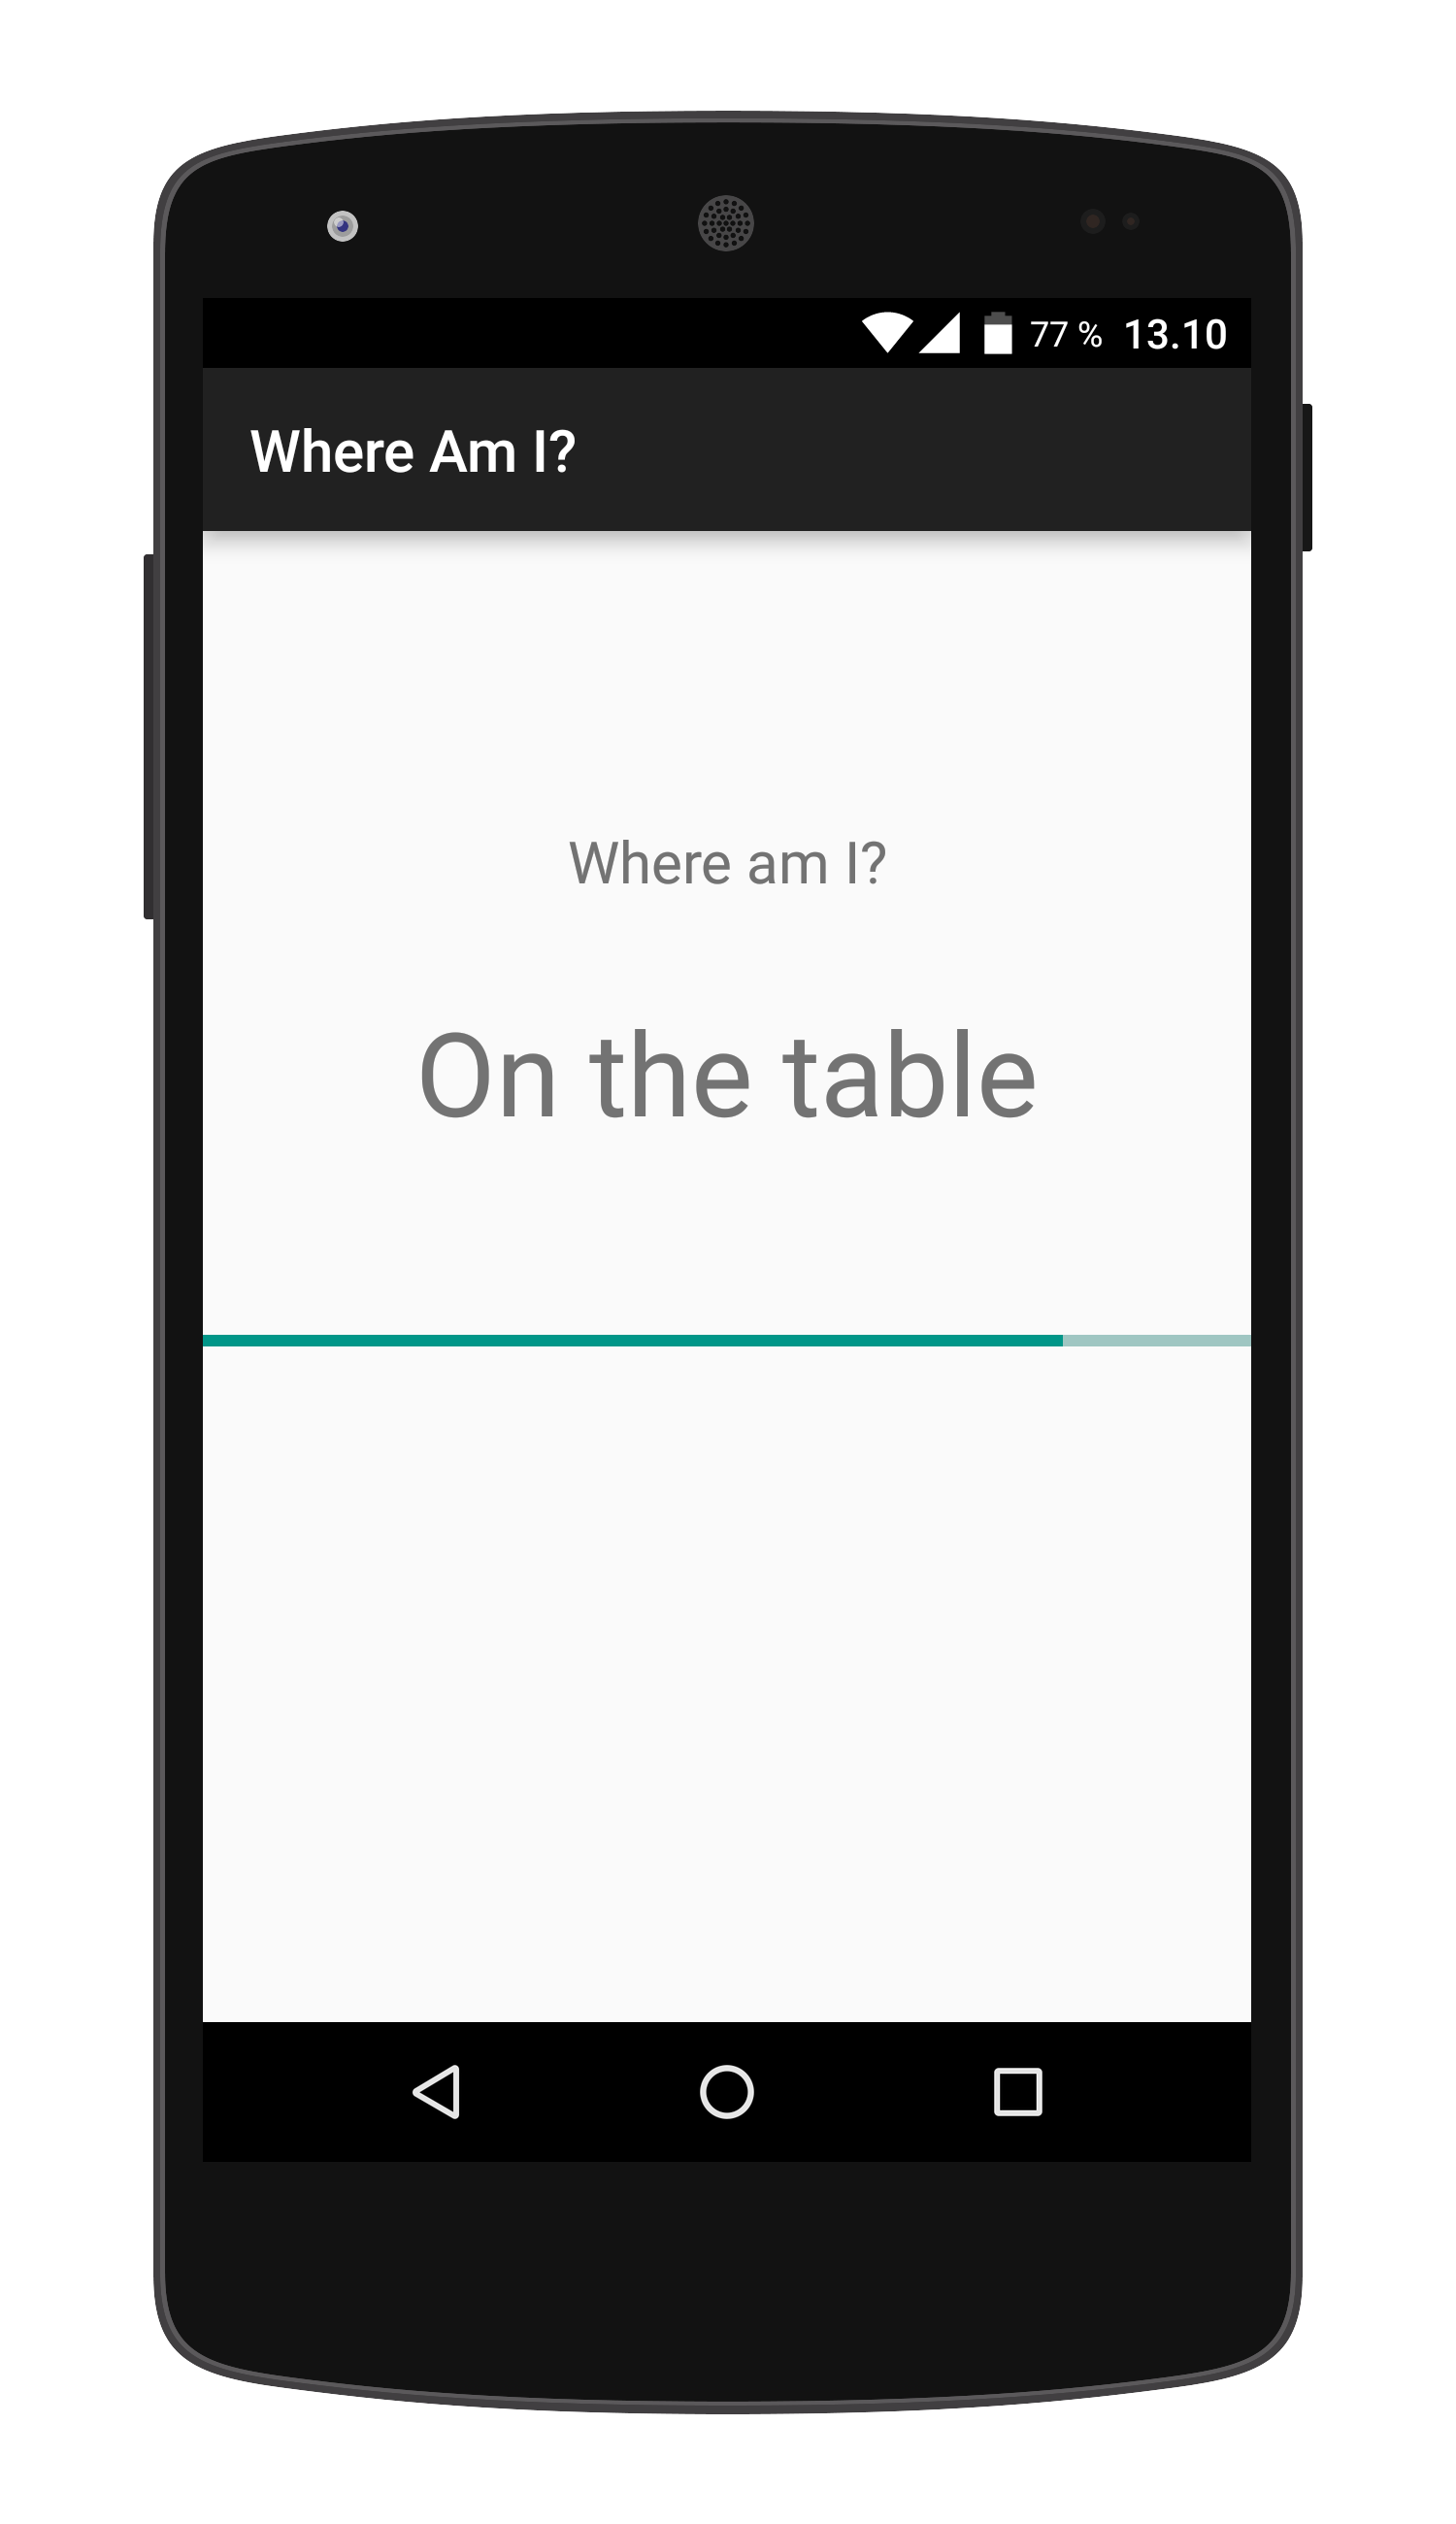
\includegraphics[width=.35\textwidth ]{graphic/quality_assurance/where_am_i_app.png}
    \caption{The example \emph{Where Am I?} application.}
    \label{fig:where_am_i_app}
\end{figure}
\FloatBarrier

The \emph{Where Am I?}-application continuously guesses if the phone is placed on a table or not, using an underlying Naïve Bayes classifier. The application starts up, trains the classifier using the snapshots, and then predicts the placement of the phone in real time. This classifier was implemented using a library called WEKA\footnote{https://weka.wikispaces.com/}, which has some predefined methods and data types that makes it relatively easy to implement a Naïve Bayes classifier.
\\\\
We found it pretty effortless to implement an application that has some notion of the context in which it exist, given our snapshots and the WEKA machine intelligence library. We spent roughly 16 man hours on the creation and execution of a campaign, and on implementing features that allow this application to parse the gathered snapshots, train a model, and display the prediction in a simple interface. We assume it would be possible to create more advanced models or classifiers, e.g. a neural network, with the data gathered from uMiner.
